\documentclass[handout]{beamer}
\usepackage{multicol}
\usepackage{xy}
\everymath{\displaystyle}
\mode<presentation>
{\usetheme{Warsaw}\setbeamercovered{dynamic}}
\usecolortheme{crane}
\usepackage{beamerfoils}
\pgfdeclareimage[height=1in]{university-logo}{ISULogo}
\logo{\pgfuseimage{university-logo}}
\setbeamertemplate{navigation symbols}{}
\title[\S6]{Section 6\\{\em And} and {\em or} problems}
\author{Dr Marcus Bishop}
\subject{Math 104}
\beamerdefaultoverlayspecification{<+->}
\theoremstyle{definition}
\newtheorem{remark}{Remark}
\newtheorem{impact}{Impact}
\newtheorem{notation}{Notation}
\newtheorem{warmup}{Warmup}
\usepackage{arev}
\begin{document}
\begin{frame}\titlepage\end{frame}
\LogoOff

\begin{frame}
\begin{warmup}
How many cards \alert{either} are picture cards \alert{or} have
suit \alert{$\varheart$}?
\end{warmup}
\begin{itemize}
\item Observe that thirteen cards have
suit \alert{$\varheart$}, namely
\[A\alert{\varheart},
2\alert{\varheart},
3\alert{\varheart},\ldots,
10\alert{\varheart},
J\alert{\varheart},
Q\alert{\varheart},
K\alert{\varheart}\]
\item Observe that twelve cards are picture cards, namely
\[J\alert{\varheart},J\alert{\vardiamond},J\clubsuit,J\spadesuit,
Q\alert{\varheart},Q\alert{\vardiamond},Q\clubsuit,Q\spadesuit,
K\alert{\varheart},K\alert{\vardiamond},K\clubsuit,K\spadesuit\]
\item However, \alert{three} cards in both groups,
namely
\[J\alert{\varheart},Q\alert{\varheart},K\alert{\varheart}\]
\item Thus $13+12-3=22$ cards are either picture cards or have 
suit \alert{$\varheart$}
\end{itemize}
\end{frame}

\begin{frame}{Union, intersection, size}
\begin{itemize}
\item Suppose $E,F$ are sets
\item $E\cup F$ denotes set of all elements of \alert{either}
$E$ \alert{or} $F$ (or \alert{both})
\item $E\cup F$ called the \alert{union} of $E$ and $F$
\item $E\cap F$ denotes set of all elements in \alert{both}
$E$ \alert{and} $F$
\item $E\cap F$ called the \alert{intersection} of $E$ and $F$
\item $\left|E\right|$ denotes number of elements,
or \alert{size} of $E$
\end{itemize}
\begin{example}
\begin{itemize}
\item Suppose $E=\left\{1,2,4\right\}$
\item Suppose $F=\left\{1,3,4\right\}$
\item Then $\left|E\right|=3=\left|F\right|$
\item $E\cup F=\left\{1,2,3,4\right\}$
\item $F\cap F=\left\{1,4\right\}$
\end{itemize}
\end{example}
\end{frame}

\begin{frame}{Example}
\begin{align*}
\only<+->{
\text{Suppose}\qquad E&=\left\{a,b,e,f\right\}\\
F&=\left\{b,c,d,f,g\right\}\\
G&=\left\{a,c,f,g\right\}\\}
\only<+->{
\text{Then}\qquad\left(E\cap F\right)\cup G}
\only<+->{
&=\left\{b,f\right\}\cup G\\}
\only<+->{
&=\left\{a,b,c,f,g\right\}\\}
\only<+->{
\left(E\cup G\right)\cap\left(F\cup G\right)}
\only<+->{
&=\left\{a,b,c,e,f,g\right\}\cap\left(F\cup G\right)\\}
\only<+->{
&=\left\{a,b,c,e,f,g\right\}\cap\left\{a,b,c,d,f,g\right\}\\}
\only<+->{
&=\left\{a,b,c,f,g\right\}}
\end{align*}
\only<+->{
\begin{remark}
In general $\left(E\cap F\right)\cup G
=\left(E\cup G\right)\cap\left(F\cup G\right)$
for any sets $E,F,G$
\end{remark}}
\end{frame}

\begin{frame}{Remarks}
\begin{itemize}
\item Order that elements \alert{of set} listed unimportant
\begin{example}
$\left\{1,2,4\right\}=\left\{4,2,1\right\}=\left\{2,1,4\right\}$
\end{example}
\item Size refers to number of \alert{distinct} elements
of set
\item If an element listed more than once, duplicates should
be eliminated before counting
\begin{example}
\begin{itemize}
\item Suppose $E=\left\{1,1,2,4,1\right\}$
\item Then $E$ the same set as $\left\{1,2,4\right\}$
\item So $\left|E\right|=3$, not $5$
\end{itemize}
\end{example}
\item Of course, would be inefficient to list
an element more than once
\end{itemize}
\end{frame}

\begin{frame}{Inclusion-Exclusion Formula}
\begin{theorem}[Inclusion-Exclusion Formula]
Suppose that
\begin{itemize}
\item $M$ has $m$ elements 
\item $N$ has $n$ elements
\item There are $p$ elements in \alert{both} $M$ and $N$
\end{itemize}
Then there are $m+n-p$ elements in \alert{either} $M$ or $N$
\end{theorem}
\end{frame}

\begin{frame}{Example}
\begin{itemize}
\item How many of $1,2,\ldots,12$ are
either divisible by $3$ or greater than $6$?
\item Numbers divisible by $3$: $3,6,9,12$
\item Numbers greater than $6$: $7,8,9,10,11,12$
\item Numbers in both groups: $9,12$
\item Thus $4+6-2=8$
either divisible by $3$ or greater than $6$?
\end{itemize}
\end{frame}

\begin{frame}{Venn diagrams}
\begin{itemize}
\item Can visualize last example using Venn diagram:
\[\begin{xy}<1cm,0cm>:
(-1,0)*\cir<2cm>{};
(1,0)*\cir<2cm>{};
(-1.5,1)*{3};
(-1.5,-1)*{6};
(0,1)*{9};
(0,-1)*{12};
(1.25,1)*{7};
(1.25,-1)*{10};
(2,1)*{8};
(2,-1)*{11};
\end{xy}\]
\item Numbers divisible by $3$ in left circle
\item Numbers greater than $6$ in right circle
\item Numbers in both groups in both circles
\end{itemize}
\end{frame}

\begin{frame}{Greek, Roman, Russian alphabets}
\begin{multicols}{2}
\begin{itemize}
\item Upper left circle shows letters of Greek alphabet
\item Upper right circle shows letters of Roman alphabet
\item Lower circle shows letters of Russian alphabet
\item How many in Roman and Russian but not Greek?
\only<+->{One, namely C}
\item How many letters in all three?
\only<+->{11}
\end{itemize}
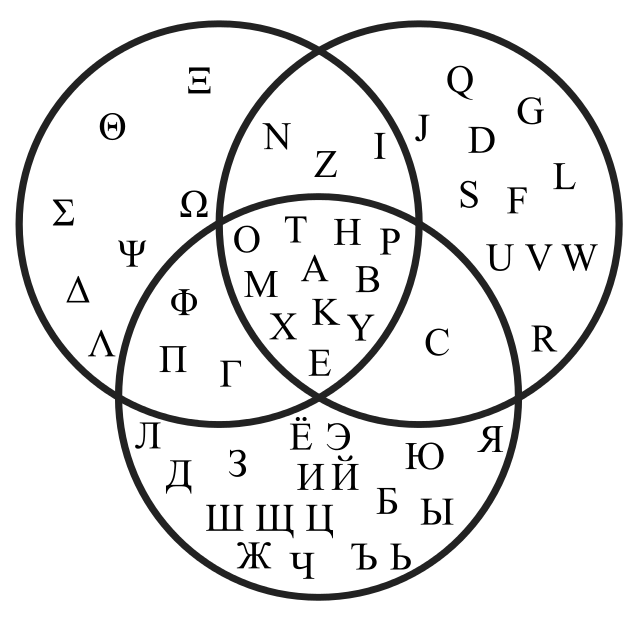
\includegraphics[scale=.25]{Venn}
\end{multicols}
\end{frame}

\begin{frame}{Freshman music majors}
\begin{itemize}
\item $100$ freshman majoring in (instrumental) music
required to be in either band or orchestra
\item $75$ in band
\item $35$ in both band and orchestra
\item How many in orchestra?
\item Rather than drawing freshmen in circles,
write only \alert{number} of freshman in each
group in corresponding region 
\[\begin{xy}<1cm,0cm>:
(-1,2)*+!D{\text{Band}};
(1,2)*+!D{\text{Orch}};
(-1,0)*\cir<2cm>{};
(1,0)*\cir<2cm>{};
(0,0)*{35};
\end{xy}\]
\end{itemize}
\end{frame}

\begin{frame}
\begin{itemize}
\item Since $75$ in band, must have
$40$ in band but not orchestra:
\[\begin{xy}<1cm,0cm>:
(-1,2)*+!D{\text{Band}};
(1,2)*+!D{\text{Orch}};
(-1,0)*\cir<2cm>{};
(1,0)*\cir<2cm>{};
(0,0)*{35};
(-2,0)*{40};
\end{xy}\]
\end{itemize}
\end{frame}

\begin{frame}
\begin{itemize}
\item Must be $100-75=25$ in orchestra but not band:
\[\begin{xy}<1cm,0cm>:
(-1,2)*+!D{\text{Band}};
(1,2)*+!D{\text{Orch}};
(-1,0)*\cir<2cm>{};
(1,0)*\cir<2cm>{};
(0,0)*{35};
(-2,0)*{40};
(2,0)*{25};
\end{xy}\]
\item Thus $35+25=60$ in orchestra
\end{itemize}
\begin{remark}
Solving Inclusion Exclusion Formula
\[75+n-35=100\]
for $n$ obviates Venn diagram
\end{remark}
\end{frame}

\begin{frame}{More Inclusion-Exclusion}
\begin{theorem}[Inclusion-Exclusion Formula]
If $E,F$ events and
\begin{itemize}
\item $p=P\left(E\right)$
\item $q=P\left(F\right)$
\item $r$ the probability that \alert{both} $E$ and $F$ occur
\end{itemize}
then $p+q-r$ the probability that \alert{either} $E$ or $F$ occurs
\end{theorem}
\begin{example}[Exercise 11]
\begin{itemize}
\item Suppose $P\left(E\right)=0.8$,
$P\left(F\right)=0.4$, and $P\left(\text{$E$ and $F$}\right)=0.5$
\item Then $P\left(\text{$E$ or $F$}\right)
=0.8+0.4-0.5=0.7$
\item Example doesn't even require context
\end{itemize}
\end{example}
\end{frame}

\begin{frame}{Example}
\begin{itemize}
\item Recall that $3,6,9,12$ divisible by $3$
\item So if number randomly selected from
$1,2,\ldots,12$ then $4/12$
the probability number divisible by $3$
\item Similarly $7,8,9,10,11,12$ greater than $6$
\item So $6/12$ the probability number
greater than $6$
\item Finally, $9,12$ divisible by $3$ \alert{and}
greater than $6$
\item So $2/12$ the probability that number
both divisible by $3$ and greater than $6$
\item By Inclusion-Exclusion
\[\frac{4}{12}+\frac{6}{12}-\frac{2}{12}=\frac{8}{12}\]
the probability
that number \alert{either} divisible by $3$ or greater than $6$
\item Indeed eight numbers $3,6,7,8,9,10,11,12$ 
divisible by $3$ or greater than $6$
\end{itemize}
\end{frame}

\begin{frame}{Mutually exclusive events}
\begin{itemize}
\item If $0=P\left(\text{$E$ and $F$}\right)$
then $E,F$ called \alert{mutually exclusive events}
\item Means that impossible for \alert{both} $E$ and $F$ to occur
\end{itemize}
\begin{example}
\begin{itemize}
\item Experiment: roll die
\item $E=\left\{1,3,5\right\}$, the event
that odd number rolled
\item $F=\left\{2,4,6\right\}$, the event
that even number rolled
\item Then $E,F$ mutually exclusive
\item Note that as sets, $E,F$ have \alert{no elements} in common
\end{itemize}
\end{example}
\begin{example}
\begin{itemize}
\item But mutually exclusive events need not be \alert{complementary}
\item $E=\left\{1,3,5\right\}$ and $F=\left\{2\right\}$
mutually exclusive
\end{itemize}
\end{example}
\end{frame}

\begin{frame}
\begin{itemize}
\item Note that if $E,F$ mutually exclusive then Inclusion-Exclusion
formula reduces to
\[P\left(\text{$E$ or $F$}\right)=P\left(E\right)
+P\left(F\right)\alert{-0}\]
since $0=P\left(\text{$E$ and $F$}\right)$
\end{itemize}
\begin{example}
\begin{itemize}
\item Experiment: randomly select card
\item $P\left(\clubsuit\right)=\frac{1}{4}=P\left(\alert{\varheart}\right)$
\item $\clubsuit,\alert{\varheart}$ mutually exclusive
since no card has \alert{both} suits
\item Thus $P\left(\text{$\clubsuit$ or $\alert{\varheart}$}\right)
=\frac{1}{4}+\frac{1}{4}=\frac{1}{2}$
\end{itemize}
\end{example}
\end{frame}

\begin{frame}{Independence}
\begin{definition}
$E,F$ called \alert{independent} if $E$
occurring or not has no effect on $F$ occurring or not
\end{definition}
\begin{example}
\begin{itemize}
\item Experiment: flip two coins
\item $E$: first coin lands on heads
\item $F$: second coin lands on heads
\item Then $E,F$ independent
\item Note that 
\[P\left(\text{$E$ and $F$}\right)=P\left(HH\right)
=\frac{1}{4}
=\frac{1}{2}\cdot\frac{1}{2}=P\left(E\right)P\left(F\right)\]
\end{itemize}
\end{example}
\end{frame}

\begin{frame}
\begin{example}
\begin{itemize}
\item Experiment: Draw two cards without replacement
\item $E$: First card has suit $\clubsuit$
\item $F$: Second card has suit $\clubsuit$
\item Then $E,F$ \alert{not} independent!
\item Indeed, $F$ occurring depends on whether or not
$E$ occurred!
\item If $E$ occurs, then $P\left(F\right)=\frac{12}{51}$
since $12$ of remaining $51$ cards have suit $\clubsuit$
\item However if $E$ fails to occur, then $P\left(F\right)=\frac{13}{51}$
since $13$ of remaining $51$ cards have suit $\clubsuit$
\end{itemize}
\end{example}
\end{frame}

\begin{frame}{Independence and \em{and}}
\begin{theorem}
If $E,F$ independent, then
$P\left(\text{$E$ and $F$}\right)=P\left(E\right)P\left(F\right)$
\end{theorem}
\begin{example}
\begin{itemize}
\item Suppose family plans to have two children
\item Calculate probability that both children girls
\item $E_1=\left\{\text{first child girl}\right\}$
\item $E_2=\left\{\text{second child girl}\right\}$
\item Then $E_1,E_2$ independent
\item $P\left(E_1\right)=1/2=P\left(E_2\right)$ so
\end{itemize}
\only<+->{
\begin{multline*}
P\left\{\text{both children girls}\right\}
\only<+->{=P\left(\text{$E_1$ and $E_2$}\right)\\}
\only<+->{=P\left(E_1\right)P\left(E_2\right)}
\only<+->{=\frac{1}{2}\cdot\frac{1}{2}}
\only<+->{=\frac{1}{4}}
\end{multline*}}
\end{example}
\end{frame}

\begin{frame}{Children continued}
\begin{itemize}
\item Suppose family plans to have \alert{ten} children
\item Calculate probability that all ten children girls
\item $E_1=\left\{\text{first child girl}\right\},\ldots,
E_{10}=\left\{\text{tenth child girl}\right\}$
\item Then $E_1,\ldots,E_{10}$ independent
\item $\frac{1}{2}=P\left(E_1\right)=P\left(E_2\right)=\cdots$
\only<+->{
\begin{multline*}
P\left\{\text{all ten children girls}\right\}
\only<+->{=P\left(\text{$E_1$ and $\cdots$ and $E_{10}$}\right)\\}
\only<+->{=P\left(E_1\right)P\left(E_2\right)\cdots P\left(E_{10}\right)}
\only<+->{=\left(\frac{1}{2}\right)^{10}}
\only<+->{=\frac{1}{1024}}
\end{multline*}}
\end{itemize}
\begin{remark}
If they succeed and decide to have another child,
$1/2$ still the probability that eleventh child a girl
\end{remark}
\end{frame}

\begin{frame}{Same problem, different story}
\begin{itemize}
\item You guess on all ten questions of true-false quiz
\item Calculate probability of answering all ten correctly
\item $E_1=\left\{\text{first question correct}\right\},\ldots,
E_{10}=\left\{\text{tenth question correct}\right\}$
\item Then $E_1,\ldots,E_{10}$ independent
and $1/2=P\left(E_1\right)=P\left(E_2\right)=\cdots$
\only<+->{\begin{multline*}
P\left\{\text{all ten questions correct}\right\}
\only<+->{=P\left(\text{$E_1$ and $\cdots$ and $E_{10}$}\right)\\}
\only<+->{=P\left(E_1\right)P\left(E_2\right)\cdots P\left(E_{10}\right)}
\only<+->{=\left(\frac{1}{2}\right)^{10}}
\only<+->{=\frac{1}{1024}}
\end{multline*}}
\item By same argument $\frac{1}{1024}$ also the probability
of answering all questions \alert{incorrectly}
\item So $\frac{1023}{1024}$ the probability of
\alert{not} answering every question incorrectly!
\end{itemize}
\end{frame}

\begin{frame}{Further variation}
\begin{itemize}
\item You guess on all ten questions of multiple choice quiz
\item All ten questions have five choices
\item Calculate probability of answering all ten correctly
\item $\frac{1}{5}=P\left(E_1\right)=P\left(E_2\right)=\cdots$ so
\only<+->{
\begin{multline*}
P\left\{\text{all ten questions correct}\right\}
\only<+->{=P\left(\text{$E_1$ and $\cdots$ and $E_{10}$}\right)\\}
\only<+->{=P\left(E_1\right)P\left(E_2\right)\cdots P\left(E_{10}\right)}
\only<+->{=\left(\frac{1}{5}\right)^{10}}
\only<+->{=\frac{1}{9765625}}
\end{multline*}}
\end{itemize}
\begin{remark}
\begin{itemize}
\item Most people would be happy with seven or eight correct
\item More difficult to compute, see \S11
\end{itemize}
\end{remark}
\end{frame}

\begin{frame}{$\clubsuit$ example revisited}
\begin{itemize}
\item Experiment: Draw two cards without replacement
\item $E$: First card has suit $\clubsuit$
\item $F$: Second card has suit $\clubsuit$
\begin{remark}
\begin{itemize}
\item We interpret \alert{$E$ and $F$} to mean $E$ occurs
\alert{and then} $F$ occurs
\item Thus we assume $E$ has already occurred when considering $F$
\item In this sense, $E,F$ \alert{independent} for purpose of calculating
$P\left(\text{$E$ and $F$}\right)$, so
$P\left(\text{$E$ and $F$}\right)=P\left(E\right)P\left(F\right)$
\end{itemize}
\end{remark}
\item $P\left(E\right)=\frac{13}{52}$
\item $E$ having occurred, $P\left(F\right)=\frac{12}{51}$
\item Thus $P\left(\text{$E$ and $F$}\right)
\only<+->{=\frac{13}{52}\cdot\frac{12}{51}}
\only<+->{=\frac{156}{2652}}\only<+->{=\frac{1}{17}}$
\end{itemize}
\end{frame}

\begin{frame}{Birthday problem}
\begin{itemize}
\item $E$: Two people in room of $24$ have same birthday
\item Calculate $P\left(E\right)$
\item Problem very complicated
\item Simpler to calculate $P\left(\text{not $E$}\right)$
\item That is, calculate probability that all $24$ people
have different birthdays
\item Second person has probability $\frac{364}{365}$ of
not having same birthday as first
\item Third person has probability $\frac{363}{365}$ of
not having same birthday as first or second
\[\frac{364}{365}
\cdot\frac{363}{365}
\cdots\frac{342}{365}\approx 0.462\]
\item So $P\left(E\right)=1-0.462=0.538$ (\alert{!})
\end{itemize}
\end{frame}

\begin{frame}{Summary}
\begin{enumerate}
\item If $E,F$ mutually exclusive then
$P\left(\text{$E$ or $F$}\right)=P\left(E\right)+P\left(F\right)$
\begin{example} $1/4+1/4$ the probability
of drawing $\clubsuit$ or $\alert{\varheart}$ \end{example}
\item If $E,F$ \alert{not} mutually exclusive then
$P\left(\text{$E$ or $F$}\right)=P\left(E\right)+P\left(F\right)
-P\left(\text{$E$ and $F$}\right)$
\begin{example} $1/4+1/13-1/52$ the probability
of drawing $\alert{\varheart}$ or a King\end{example}
\item If $E,F$ independent then
$P\left(\text{$E$ and $F$}\right)=P\left(E\right)P\left(F\right)$
\begin{example} $\left(1/2\right)\left(1/2\right)$ the probability
of both coins landing on heads\end{example}
\end{enumerate}
\end{frame}

%\begin{frame}{Quiz instructions}
%\begin{itemize}
%\item First submit homework \alert{without fringe}
%\item Use number 2 pencil
%\item No phones
%\item Fill in student ID in \alert{first nine spaces},
%leaving tenth space empty
%\item Leave when finished, depositing quiz and answer sheet
%face-down on table in back
%\item Yellow and red forms of quiz in \alert{different piles}
%\end{itemize}
%\end{frame}
\end{document}
